\documentclass[a4paper,11pt]{article}
\usepackage[utf8]{inputenc}
\usepackage[T1]{fontenc}
\usepackage{graphicx}
\usepackage{geometry}
\usepackage[colorlinks,linkcolor=black,urlcolor=cyan,citecolor=cyan]{hyperref}
\usepackage{amsmath}
\usepackage{fancyhdr}
\usepackage{float}
\usepackage{listings}
\usepackage{tikz}
\usepackage{animate}

\usepackage{xcolor}
\usepackage[french]{babel}

\geometry{left=3cm,right=3cm,top=2.5cm,bottom=2.5cm}

\hypersetup{
    colorlinks=true,
    linkcolor=black,
    urlcolor=cyan,
    citecolor=cyan
}

\lstset{
    language=Fortran,
    basicstyle=\tiny,
    keywordstyle=\color{blue}\bfseries,
    commentstyle=\color{gray},
    stringstyle=\color{red},
    numbers=left,
    numberstyle=\tiny\color{gray},
    stepnumber=1,
    breaklines=true,
    frame=single,
    captionpos=b,
    tabsize=4,
    showstringspaces=false,
}

\begin{document}



\begin{titlepage}
    \begin{figure}
        
\includegraphics[width=0.4\linewidth]{images/logo_em.jpg}
    \end{figure}
    \begin{center}
        \vspace*{3.5cm}


        \huge \textbf{Travail d'étude et de Recherche} \\
        Compte rendu du Semestre 5
        \vspace{1cm}

        \hrulefill
        
        \vspace{0.4cm}
        {\Huge \textbf{Modélisation du transfert thermique et de masse dans la pyrolyse du bois}} \\
        \vspace{0.25cm}
        \hrulefill
        
        \vspace{7cm}

        \Large Année Universitaire 2024 - 2025
        
        \vspace{2cm}
        
        \normalsize
        \textbf{Participants :}
        Simon Francheo, Julien Léger, Gurwan Le Hebel, Pierre Mériaux

        \textbf{Encadrants :}
        Ludovic Godard-Cadillac, Thanh-Ha Nguyen-Bui 

        \vfill
        
    \end{center}
\end{titlepage}

\newpage
\tableofcontents
\newpage

\pagestyle{fancy}
\fancyhead{}
\fancyhead[L]{TER - Pyrolyse du bois}
\fancyhead[R]{23 Janvier 2025}


\section{Introduction}
La construction d'un modèle de comportement de la pyrolyse du bois est un enjeu pour la sécurité incendie en forêt et pour les constructions. Ce modèle doit permettre le bon dimensionnement des structures en anticipant la formation d'une couche de charbon isolante autour du bois sain. 
\\

Le modèle que nous étudions utilise le couplage d'une modélisation des réactions chimiques de pyrolyse et d'une modélisation de la diffusion de la chaleur. La \nameref{sec:theo} présente les hypothèses, les équations utilisées et leurs schémas numériques. La résolution des équations sur les masses volumiques est ensuite effectuée en comparant les schémas Euler implicite et Crank-Nicolson. Le choix de schémas implicites est dû à des raisons de stabilité, d'absence de condition CFL contraignante sur le pas de temps et est facilité par la possibilité d'inverser analytiquement le schéma. Concernant la résolution de l'équation de la chaleur, un schéma numérique implicite est choisi, résultant d'un compromis entre temps de calcul et stabilité du schéma.


\section{Partie théorique}\label{sec:theo}

La réaction de combustion est modélisée par un système d'équations différentielles qui repose sur la conservation de masse du bois \cite{1}, du charbon, du gaz, du liquide et de la vapeur au cours du processus. Il s'écrit comme suit :
\begin{equation}\label{eq:1}
	\left\lbrace
		\begin{aligned}
			\frac{\partial \rho_b}{\partial t} &= -(k_1 + k_2)\rho_b \\
                \frac{\partial \rho_c}{\partial t} &= k_1\rho_b\\
                \frac{\partial \rho_g}{\partial t} &= k_2\rho_b\\
                \frac{\partial \rho_l}{\partial t} &= -k_3\rho_l\\
                \frac{\partial \rho_v}{\partial t} &= k_3\rho_l\\
		\end{aligned}
	\right.
\end{equation}

où $\rho_b, \rho_c, \rho_g, \rho_l, \rho_v$ sont respectivement les masses volumiques du bois, du charbon, du gaz, du liquide et de la vapeur.

$k_1, k_2, k_3$ sont les taux de réactions chimiques de la pyrolyse du bois humide. Ceux-ci sont décrits par la loi d'Arrhenius \cite{1}: 
\begin{equation}\label{eq:2}
    k_i = A_i\exp{\left(\frac{-E_i}{RT}\right)}, i = 1,2,3
\end{equation}

où $A_i$ sont des constantes de réactions, $E_i$ les énergies d'activation, R la constante des gaz parfaits et enfin T la température.

L'objectif est de résoudre ce système d'équations numériquement grâce à différents schémas implicites. Les applications numériques seront réalisées à partir de différentes essences de bois mouillés (cf \cite{1}). La relation suivante permet à partir des données brutes sur l'essence de bois étudiée d'extraite les masses volumiques $\rho_{b_0}$ et $\rho_{l_0}$ initiale \cite{1}.

\begin{equation}\label{eq:3}
    \rho_0 = (1 - \chi)\rho_{b_0} + \chi\rho_{l_0}
\end{equation}

où $\rho_0$ est la masse volumique du bois sec, et $\chi$ le taux d'humidité du bois. \\


Pour impliciter nos schémas numériques, il faut remarquer que les variations de $\rho_c, \rho_g$ sont dépendants uniquement de $\rho_b$, même chose pour $\rho_v$ qui dépend de $\rho_l$. Il faut inverser les équations pour $\rho_b$ et $\rho_l$ afin d'en déduire les autres avec les formules usuelles du schéma choisi. Les schémas sont alors partiellement implicites. Cette technique permet par exemple d'éviter l'utilisation de la méthode de Newton qui est très exigeante en temps de calcul. Le schéma numérique de Euler implicite s'écrit alors comme suit pour résoudre le système \eqref{eq:1}:

\begin{equation}\label{eq:EI}
	\left\lbrace
		\begin{aligned}
			\rho_b^{n+1} &=  \frac{\rho_b^n}{1 + \Delta t(k_1^{n+1}+k_2^{n+1})} \\
                \rho_c^{n+1} &= \rho_c^n + \Delta t \cdot k_1^{n+1} \rho_b^{n+1}\\
                \rho_g^{n+1} &= \rho_g^n + \Delta t \cdot k_2^{n+1}\rho_b^{n+1}\\
                \rho_l^{n+1} &= \frac{\rho_l^n}{1 + \Delta t \cdot k_3^{n+1}} \\
                \rho_v^{n+1} &= \rho_v^n + \Delta t \cdot k_3^{n+1} \rho_l^{n+1} \\
		\end{aligned}
	\right.
\end{equation}


Inversé analytiquement, le schéma de Crank-Nicolson implicite pour notre système s'écrit :

\begin{equation}\label{eq:CK}
	\left\lbrace
		\begin{aligned}
			\rho_b^{n+1} &= \rho_b^n \left( \frac{1 - \frac{\Delta t}{2}(k_1^n + k_2^n) }{1 +\frac{\Delta t}{2}(k_1^{n+1} + k_2^{n+1}) }\right)  \\
                \rho_c^{n+1} &= \rho_c^n + \frac{\Delta t}{2} \left( k_1^{n+1} \rho_b^{n+1} + k_1^n \rho_b^n \right) \\
                \rho_g^{n+1} &= \rho_g^n + \frac{\Delta t}{2} \left( k_2^{n+1} \rho_b^{n+1} + k_2^n \rho_b^n \right) \\
                \rho_l^{n+1} &= \rho_l^n \left(\frac{ 1 - \frac{\Delta t}{2} \cdot k_3^n }{ 1 + \frac{\Delta t}{2} \cdot k_3^{n+1} }\right)  \\
                \rho_v^{n+1} &= \rho_v^n + \frac{\Delta t}{2} \left( k_3^{n+1} \rho_l^{n+1} + k_3^n \rho_l^n \right) \\
		\end{aligned}
	\right.
\end{equation}

\section{Introduction}

\section*{Schéma Euler Implicite 1D}

\[
- \beta_{i-1}^{n} T_{i-1}^{n+1} + (1 + \alpha_i^n) T_i^{n+1} - \beta_{i+1}^{n} T_{i+1}^{n+1} = T_i^n + \gamma_i^n Q_i^n
\]

\[
\beta_{i \pm 1}^{n} = \frac{\Delta t}{\Delta x^2} \frac{\lambda_{i \pm \frac{1}{2}}^n}{(\rho C_p)_i^n}
\]

\[
\alpha_i^n = \frac{\Delta t}{\Delta x^2 (\rho C_p)_i^n} \left( \lambda_{i - \frac{1}{2}}^n + \lambda_{i + \frac{1}{2}}^n \right)
\]

\[
\gamma_i^n = \frac{\Delta t}{(\rho C_p)_i^n}
\]

\subsection*{Forme Matricielle}

\[
(I + A) \cdot T^{n+1} = b
\]

où $\mathbf{A}$ est une matrice tridiagonale et b un vecteur:

\[
\mathbf{A} =
\begin{bmatrix}
\alpha_1^n & -\beta_2^n & 0 & \cdots & 0 \\
-\beta_1^n & \alpha_2^n & -\beta_3^n & \cdots & 0 \\
0 & \ddots & \ddots & \ddots & 0 \\
\vdots & \cdots & -\beta_{Nx-2}^n & \alpha_{Nx-1}^n & -\beta_{Nx}^n \\
0 & \cdots & 0 & -\beta_{Nx-1}^n & \beta_{Nx}^n
\end{bmatrix}
,\quad
b =
\begin{bmatrix}
    T_1^n + \beta_{0}^n T_0^n + \gamma_1^nQ_1^n \\
    T_2^n + \gamma_2^nQ_2^n  \\
    \vdots \\
    \vdots \\
    T_{Nx}^n + \gamma_{Nx}^nQ_{Nx}^n 
    
\end{bmatrix}
\]

\section*{Schéma Crank-Nicolson 1D}

\[
- \frac{\beta_{i-1}^{n}}{2} T_{i-1}^{n+1} + \left(1 + \frac{\alpha_i^n}{2} \right) T_i^{n+1} - \frac{\beta_{i+1}^n}{2} T_{i+1}^{n+1} =
\frac{\beta_{i-1}^n}{2} T_{i-1}^{n} + \left(1 - \frac{\alpha_i^n}{2} \right) T_i^{n} + \frac{\beta_{i+1}^n}{2} T_{i+1}^{n} + \gamma_i^n Q_i^n
\]

\subsection*{Forme Matricielle}

\[
(I + \frac{1}{2}A) \cdot T^{n+1} = (I - \frac{1}{2}A) \cdot T^n + \gamma^n \cdot Q^n 
\]
\vspace{0.5cm}

\section*{Schéma Euler Implicite 2D}

\[
(1 + \alpha_{i,j}^n) T_{i,j}^{n+1} = T_{i,j}^{n} + \beta_{i+1}^{n} T_{i+1,j}^{n+1} + \beta_{i-1}^{n} T_{i-1,j}^{n+1} + \beta_{j+1}^{n} T_{i,j+1}^{n+1} + \beta_{j-1}^{n} T_{i,j-1}^{n+1} + \gamma_{i,j}^n Q_{i,j}^n
\]

\[
\beta_{i\pm1}^n = \frac{\Delta t}{\Delta x^2} \frac{\lambda_{i \pm \frac{1}{2}, j}^n}{(\rho C_p)_{i,j}^n}
\qquad
\beta_{j\pm1}^n = \frac{\Delta t}{\Delta y^2} \frac{\lambda_{i, j \pm \frac{1}{2}}^n}{(\rho C_p)_{i,j}^n}
\]

\[
\alpha_{i,j}^n = \beta_{i-1}^n + \beta_{i+1}^n + \beta_{j-1}^n + \beta_{j+1}^n
\qquad
\gamma_{i,j}^n = \frac{\Delta t}{(\rho C_p)_{i,j}^n}
\]
\section*{Résultats et interprétations}\label{sec:ri}


\section{Partie chimie}
 
\subsection{Résolution numérique}

Pour obtenir les résultats, le temps maximal d'étude a été fixé à 300s (5 minutes), temps suffisant pour que toutes les transformations chimiques se produisent. Une température variant linéairement au cours du temps est choisie afin de ne pas compliquer le système. Cette température varie de 300K (température ambiante) à 1000K (727 °C) au cours de la réaction, permettant la visualisation de chaque transformation chimique en fonction de la température. Les taux de réactions chimiques k varient en même temps que la température, ce qui est décrit par la loi d'Arrhenius \eqref{eq:2}. En ce qui concerne la discrétisation du temps pour notre schéma numérique, le pas de temps est fixé à 0.1 s. Celui-ci est suffisamment petit pour avoir des résultats fiables (surtout avec Crank Nicolson), tout en garantissant un temps de calcul presque instantané. Le nombre d'itérations nécessaires pour le schéma N est donc de 3000. 
\\

L'essence de bois étudiée pour la résolution est principalement le Chêne de Mongolie (cf \cite{1}), celui-ci étant représentatif des charpentes utilisées dans les habitations, il est donc intéressant de le modéliser pour la prévention des incendies. \\

Pour un schéma donné, le programme principal stocke les données du problème et écrit les masses volumiques à chaque instant de notre subdivision. Cela est possible grâce à une boucle qui actualise successivement la température - donc les taux de réactions \eqref{eq:2} - et calcule les masses volumiques au temps n+1. Enfin, un script Gnuplot est utilisé pour tracer ces données :

\begin{figure}[H]
    \centering
    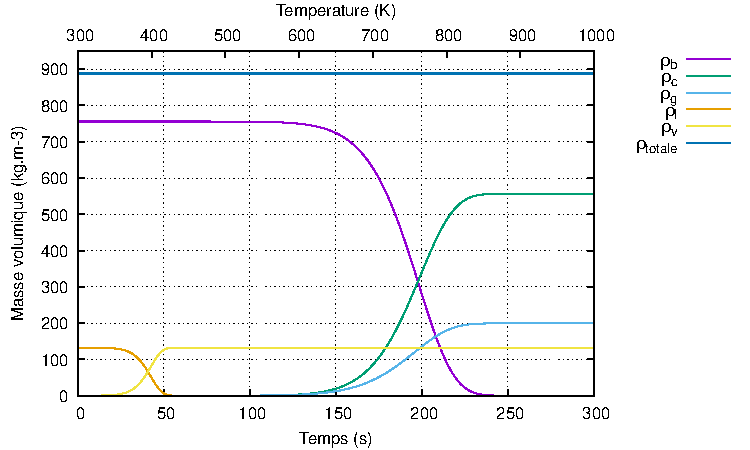
\includegraphics[width=0.95\linewidth]{images/densite_CK2.pdf}
    \caption{Évolution des masses volumiques en fonction du temps (et de la température) avec le schéma numérique de Crank Nicolson implicite }
    \label{fig:densiteCK2}
\end{figure}

L'évolution des masses volumiques correspond aux attentes suggérées par l'intuition physique. En effet, se produit dans un premier temps la vaporisation de l'eau (croisement des courbes de $\rho_l$ et $\rho_v$) autour de 100 °C. Celle-ci est suivie par la combustion, qui débute aux alentours de 600K, et qui est caractérisée par la transformation du bois en charbon et en gaz. De plus, la masse volumique totale reste stable tout au long de l'expérience. Ces observations confirment le bon comportement qualitatif du modèle.

\subsection{Étude de l'erreur}

Pour évaluer l'évolution de l'erreur locale d'un schéma en fonction du temps, on peut comparer deux solutions : l'une obtenue avec le schéma classique et l'autre avec le même schéma, mais en utilisant un pas de temps réduit, par exemple divisé par 10 (donc plus précis). L'écart absolu entre ces deux solutions à un instant donné t fournit une estimation de l'erreur locale du schéma.

\begin{figure}[H]
    \centering
    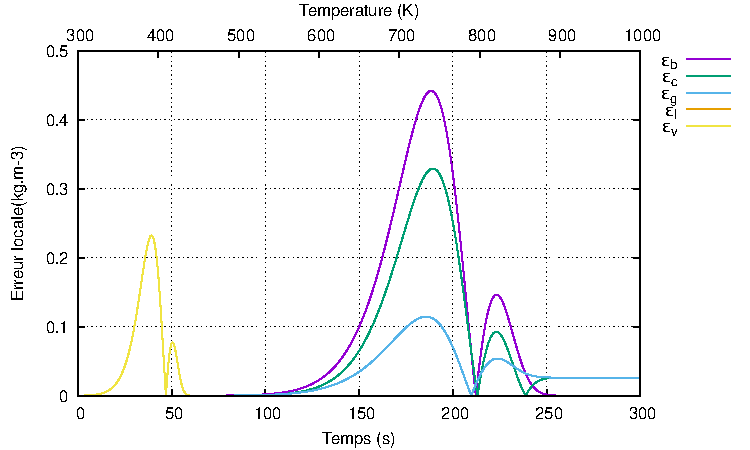
\includegraphics[width=0.9\linewidth]{images/error_EI.pdf}
    \caption{Évolution des erreurs numériques locales sur les masses volumiques en fonction du temps (et de la température) pour le schéma de Euleur implicite }
    \label{fig:erEI}
\end{figure}


\begin{figure}[H]
    \centering
    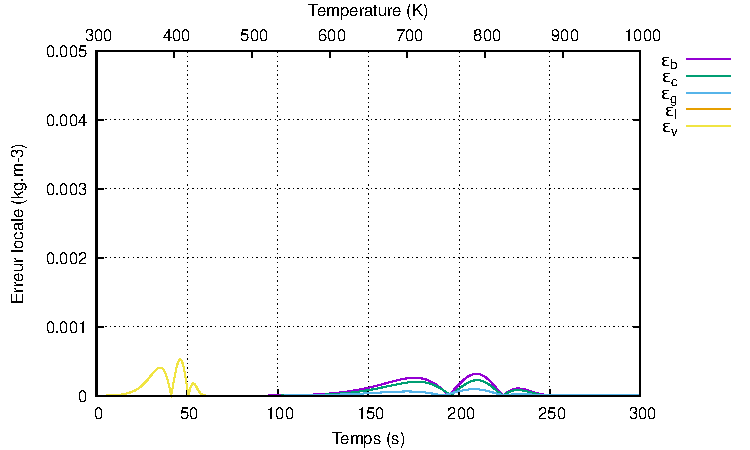
\includegraphics[width=0.9\linewidth]{images/error_CK2.pdf}
    \caption{Évolution des erreurs numériques locales sur les masses volumiques en fonction du temps (et de la température) pour le schéma de Crank Nicolson. L'échelle de l'ordonnée est 100 fois plus petite que sur le graphe de l'erreur avec le schéma d'Euler)}
    \label{fig:erCK2}
\end{figure}

L'erreur devient plus importante aux moments où les masses volumiques varient le plus. Les ordres de grandeurs des erreurs numériques commises par les deux schémas sont incomparables: 0.1 kg.m-3 pour Euler implicite, 0.0001 kg.m-3 pour Crank-Nicolson. Cela est cohérent avec le fait que le schéma de Crank-Nicolson possède un ordre plus élevé (2) que Euler implicite (1). Les temps de calculs étant inférieurs à une seconde, le schéma de Crank-Nicolson est donc préférable.

\subsection{Partie chaleur}
Dans un premier cas on se limite à un cas unidimensionnel.
On utilise l'équation de la chaleur : 
\begin{equation}\label{eq:6}
\frac{\partial T}{\partial t} =    \frac{\lambda}{ \rho C_p} \frac{\partial^2 T}{\partial x^2} + Q_r
\end{equation}

On considère $ Q_r = 0$ , $\rho C_p = 0 $, $\lambda = 0$. On impose le les conditions aux limites : $\forall t$ on prend $ T(t, x=0) = T_0$ et $T(t, x=L) = T_0$. \\

\begin{tikzpicture}
    \draw (1,0) rectangle (4,1); % Dessine un rectangle de 5x3 cm
    \draw[<->] (1, 0.5) -- (4, 0.5);
    \node at (5, 0) {$T_0$};
    \node at (0, 0) {$T_0$};
    \node at (2.5, 0.8) {$L$};   
\end{tikzpicture}

Puis on choisi comme condition initiale, une condition de Dirichlet : $T(t=0, x) = T_0 + T_{max}*sin(\pi\frac{x}{L})$.

%\begin{tikzpicture}
%\draw (4, 1) -- (4, 2) -- (8, 2) -- (8, 1) -- (4, 1);

%\end{tikzpicture}


Afin de résoudre l'équation, on utilise une méthode numérique avec 3 points en espace : 
\begin{equation}\label{eq:7}
    \frac{\partial^2 T_i}{\partial x^2}= \frac{T_{i+1}+T_{i-1}-2T_i}{\Delta x^2}
\end{equation}
Puis, celle d'Euler implicite pour le temps :

$$ \frac{T_i^{n+1}-T_i^n}{\Delta t}= \frac{T_{i+1}^n+T_{i-1}^n-2T_i^{n+1}}{\Delta x^2} $$

\begin{equation}\label{eq:8}
    T_i^{n+1}=T_i^n + \frac{D\Delta t}{\Delta x^2} ( T_{i+1}^n-2T_i^n+T_{i-1^n})
\end{equation}
Avec $D = \rho C_p$, $i$ représentent les indices d'espaces et $n$ les indices temporels.

Pour calculer l'erreur il nous est donnée l'équation, avec une initialisation avec la condition de Dirichlet : 
\begin{equation}
    T(t,x) = T_0 + T_1 sin(\pi\frac{x}{L})exp(-D(\frac{\pi}{L})^2t)
\end{equation}

On a donc pour chaque pas de temps et en un $x$ fixé 
$$ err_i^n = \mid T_i^n - T(n\Delta t, x_i) \mid. $$




\newpage

\begin{figure}
    \centering
    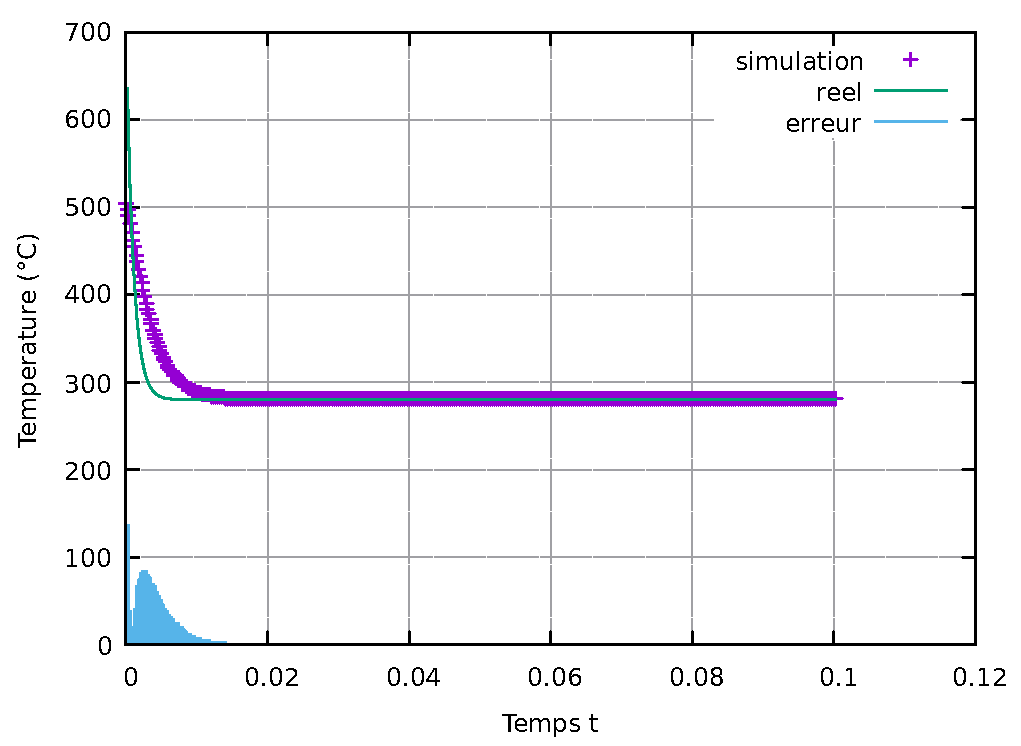
\includegraphics[width=0.9\linewidth]{images/Temperature_en_un_point.pdf}
    \caption{température en un point et l'erreur}
\end{figure}

On peut remarquer une erreur importante au début de la simulation (le pic), cela est surprenant sachant qu'à $t=0$ les données initiales sont les mêmes. En dehors de ce qui semble suspect, on atteint un maximum à $80^{\circ} C$. Ensuite, on diminue jusqu'à une erreur quasi nulle.


Lors de cette partie quelques difficultés et questions se posent. La première difficulté est la combinaison des indices d'espaces et temporels; car l'équation doit être discrétisée en espace et en temps. Après, effectué un maillage avec la température,le temps et l'espace s'avère complique, c'est pour cela que pour le moment le graphique précédent est pour un point. Ensuite, il faut savoir si une condition doit s'appliquer aux pas de temps ou d'espace pour avoir convergence. Après l'analyse de l'équation \eqref{eq:8}, on peut en déduire qu'elle est inconditionnellement stable. De plus, on peut se demander quel serait le résultat avec d'autre méthode numérique (en terme de précision et de température). Enfin, une condition de Dirichlet est utilisée ci-dessus, cependant il est possible de faire l'initialisation avec Neumann pour un milieu semi-infini.

\section{Couplage}

\subsection{1D}

\subsection{2D}

\begin{figure}[H]
    \animategraphics[autoplay, loop, width=\linewidth, controls]{5}{images/2D/temp_}{01}{41}
\end{figure}
  
\begin{figure}[H]
    \animategraphics[autoplay, loop, width=\linewidth, controls]{5}{images/2D/rho_}{01}{41}
\end{figure}
\begin{figure}[H]
\end{figure}[H]

\subsection{Conclusion}

Pour conclure, on sait que la réaction chimique dépend de la température et que le coefficient de diffusion thermique, de l'équation de la chaleur, dépend des éléments pris en compte dans le volume donné. Comme tout cela est lié, il est reste à combiner les deux approches; c'est-à-dire mettre pour chaque pas de temps l'équation en chimie avec les données de la température, puis la température en fonction des éléments chimiques présent.

\section{Objectif pour la suite du projet}

Comme vu précédemment, nous sommes désormais capable de simuler l'évolution des densités de chaque matière pendant la réaction en choisissant un profil de température donné d'un côté, et celle du profil de température à l'intérieur du bois sans prendre en compte les réactions chimiques qui interviennent. Notre but est donc à présent de combiner ces deux aspects afin d'obtenir une simulation plus fidèle à la réalité. Pour cela, nous nous appuierons sur l'équation de la chaleur :

\begin{equation}\label{eq:10}
    \frac \partial{\partial t} (\rho C_p T) = \frac{\partial}{\partial x} (\lambda \frac{\partial T}{\partial x}) + Q_r
\end{equation}

En discrétisant cette équation, on obtient le schéma implicite suivant :

\begin{equation}\label{eq:11}
	   T_i^{n+1} = \frac {(\Delta x^2 T_i^n + \Delta t (\lambda_{i+1}^n - \lambda_i^n)(T_{i+1}^n - T_i^n) + \Delta t \lambda_i^n (T_{i+1}^n + T_{i-1}^n) + \Delta x^2 \Delta t {Q_r}_i^n} {\Delta x^2 \rho {C_p}_i^n + 2\Delta t \lambda_i^n}
\end{equation}

De plus, ce schéma devra respecter certaines conditions aux limites, inhérentes à l'équation de la chaleur :

\begin{equation}\label{eq:12}
       \frac \partial {\partial t} (T(t, 0)(\rho _b C_b + \rho _c C_c + \rho _l C_l)) = \frac {(\alpha q_e (t, 0) - q_{loss} (t, 0) - \lambda (t, 0)\frac {\partial T} {\partial x} (t, 0))} {\Delta x} + Q_r(t, 0)
\end{equation}

\begin{equation}\label{eq:13}
       \frac \partial {\partial t} (T(t, L)(\rho _b C_b + \rho _c C_c + \rho _l C_l)) = \frac {(\alpha q_e (t, L) - q_{loss} (t, L) - \lambda (t, L)\frac {\partial T} {\partial x} (t, L))} {\Delta x} + Q_r(t, L)
\end{equation}

Il faudra donc également discrétiser ces équations afin de les intégrer au schéma numérique \eqref{eq:11}.
\newpage
\section{Annexes}
Ci-dessous des bouts de code en Fortran qui contiennent des procédures importantes pour ce TER, notamment celles calculant les nouvelles masses volumiques au temps n+1 ainsi que la procédure du programme principal permettant de construire nos données. Pour des raisons de clarté, la création des données pour Crank-Nicolson est omise car elle ressemble fortement à celle d'Euler.

\vspace{0.5cm}
\begin{lstlisting}[caption={Procédure \texttt{Euler\_step}}, label={lst:euler_step}]
subroutine Euler_step(rho, k, dt)

    real(PR), dimension(:), intent(inout)   :: rho, k
    real(PR), intent(in)                    :: dt

    rho(1) = rho(1)/(1._PR + dt * (k(1) + k(2)))
    rho(2) = rho(2) + dt * k(1) * rho(1)
    rho(3) = rho(3) + dt * k(2) * rho(1)
    rho(4) = rho(4)/(1._PR + dt * k(3))
    rho(5) = rho(5) + dt * k(3) * rho(4)

end subroutine Euler_step
\end{lstlisting}

\begin{lstlisting}[caption={Procédure \texttt{CK2\_step}}, label={lst:ck2_step}]
subroutine CK2_step(rho, k, k_new, dt)

    real(PR), dimension(:), intent(inout)   :: rho, k, k_new
    real(PR), intent(in)                    :: dt
    real(PR)                                :: rhob, rhol

    rhob = rho(1)
    rhol = rho(4)

    rho(1) = rho(1) * ((1._PR - dt/2._PR * (k(1) + k(2)))/(1._PR + dt/2._PR *(k_new(1) + k_new(2))))
    rho(2) = rho(2) + dt/2._PR * (k_new(1) * rho(1) + k(1) * rhob)
    rho(3) = rho(3) + dt/2._PR * (k_new(2) * rho(1) + k(2) * rhob)
    rho(4) = rho(4) * ((1._PR - dt/2._PR * k(3))/(1._PR + dt/2._PR * k_new(3)))
    rho(5) = rho(5) + dt/2._PR * (k_new(3) * rho(4) + k(3) * rhol)

end subroutine CK2_step
\end{lstlisting}

\begin{lstlisting}[caption={Procédure \texttt{create\_data\_Euler}}]
subroutine create_data_Euler(rho, k, t, tf, dt, Temp, Tempf)

    real(PR), dimension(:), intent(inout)   :: rho, k                   !Vecteurs contenant les masses volumiques et taux de reactions du systeme
    real(PR), intent(inout)                 :: t, tf, dt, Temp, Tempf   !temps (initialement 0), temps final, pas de temps, temperature (initialement 300K), temperature finale 
                                                                        !
    real(PR)                                :: t1, t2, alpha
    integer                                 :: N, i

    open(unit=101, file = "data/densite_Euler.dat")
    
    N = INT(tf/dt) !Calcul du nombres d'operations pour le schema

    alpha = (Tempf-Temp)/tf !Alpha est le coefficient directeur de T(t)
                            !Pour aller de la temperature initiale a finale en un temps tf (t0=0)

    call cpu_time(t1)
    do i = 1, N

        write(101,*) rho, t, Temp
        Temp = Temp + dt*alpha      !Calcul de la temperature au temps t_n+1

        call arrhenius(k, Temp)     !Calcul des coefficients k au temps t_n+1
                                    !avec la loi d'Arrhenius
                                    
        call Euler_step(rho, k, dt) !Un pas de temps avec le schema implicite d'Euler
                                    !calcul de rho_n+1
        t = t + dt
    
    end do
    
    call cpu_time(t2)
    print *, "Temps d'execution Euler-SI :", t2 - t1
    close(101)

end subroutine create_data_Euler
\end{lstlisting}


\vspace{2cm}

Le schéma de l'évolution des masses volumiques en fonction du temps obtenu avec Euler implicite est presque indissociable à l'oeil nu de celui de Crank-Nicolson (Figure \ref{fig:densiteCK2}). Il est alors peu pertinent de le mettre dans la partie résultat, cela évite de surcharger le document.
\begin{figure}[H]
    \centering
    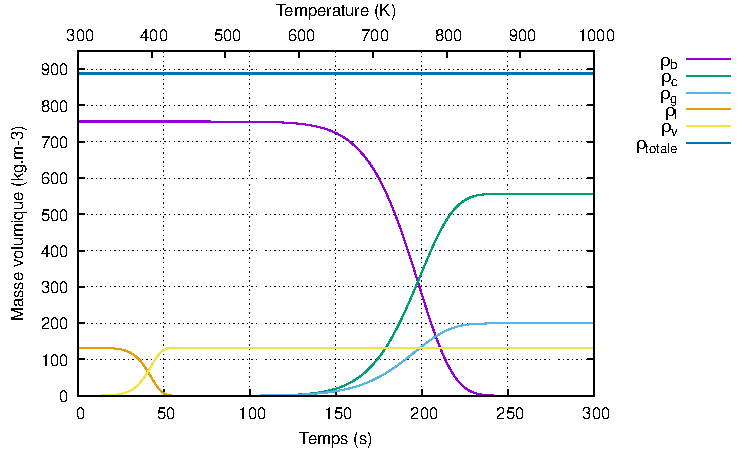
\includegraphics[width=1\linewidth]{images/densite_Euler.pdf}
    \caption{Évolution des masses volumiques en fonction du temps (et de la température) avec le schéma numérique de Euler implicite }
    \label{fig:densiteEI}
\end{figure}


\newpage
\begin{thebibliography}{99}

    \addcontentsline{toc}{section}{Bibliographie}

    \bibitem{1} D.K. Shen et al, \textit{Modeling pyrolysis of wet wood under external heat flux}, Fire Safety Journal 42 (2007) 210–217

\end{thebibliography}

\end{document}